\begin{figure}[t]
\centering
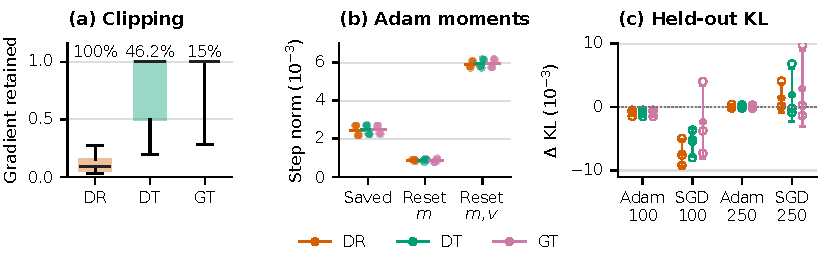
\includegraphics[width=\linewidth]{figures/added_control_figures_20260914/normalization_interventions.pdf}
\caption{\textbf{Response averaging triggers more clipping; Adam history shapes step norms and one-step loss changes.}
(a) Retained gradient fraction and clipping rates for response (DR), within-domain token (DT), and global token (GT) averaging.
(b) Step norms after resetting Adam's first moment or both moments, retaining the step count.
(c) Held-out reverse-KL changes (lower is better). Open points are the three batches per checkpoint; filled points and bars show their means and standard deviations. SGD steps match the corresponding Adam step norm.}
\label{fig:normalization_interventions}
\end{figure}
